In the adjoining figure, two circles of radii 6 and 8 are drawn with their centers 12 units apart.  At $P$, one of the points of intersection, a line is drawn in such a way that the chords $QP$ and $PR$ have equal length.  Find the square of the length of $QP$.

\begin{center}
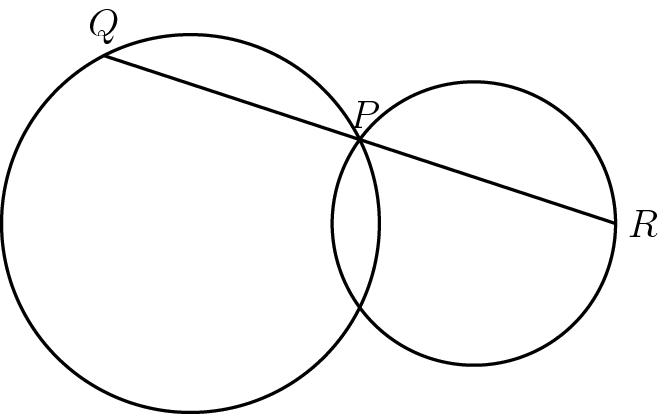
\includegraphics[width = 66.4mm]{img/fig0.png}
\end{center}